\documentclass{article}

%
% 引入模板的style文件
%
\usepackage{homework}

\setCJKmainfont{SimSun}[AutoFakeBold] %宋体加粗
\setCJKsansfont{SimHei}[AutoFakeBold] %黑体加粗


\usepackage{minted} %配合minted宏包进行好看的高亮
\usepackage{currfile} %配合minted宏包进行好看的高亮
\usepackage{caption} %配合minted宏包进行好看的高亮
\usepackage{tcolorbox} %配合minted宏包进行好看的高亮
\usepackage{xcolor} %配合minted宏包进行好看的高亮
\tcbuselibrary{skins} %配合minted宏包进行好看的高亮
\tcbuselibrary{minted} %配合minted宏包进行好看的高亮
\usemintedstyle{paraiso-dark} %配合minted宏包进行好看的高亮



%
% 封面
%

\title{
	
\includegraphics[width=0.6\textwidth]{images/title/ucas_logo 1.pdf}\\
    \vspace{1in}
    \textmd{\textbf{\hmwkClass}}\\
	\textmd{\Large{\textbf{\hmwkClassID}}}\\
    \textmd{\textbf{\hmwkTitle}}\\
    \normalsize\vspace{0.1in}\large{\hmwkCompleteTime }\\
    \vspace{0.1in}\large{\textit{\hmwkClassInstructor\ }}\\
    \vspace{1in}
	
\includegraphics[width=0.25\textwidth]{images/title/Cyber.jpg}\\
	\vspace{1in}
}


\author{
	\hmwkAuthorName \\ 
	\hmwkAuthorStuID \\
	\hmwkAuthorInst \\
	\hmwkAuthorzhuanye \\
	\hmwkAuthorfangxiang
	}
\date{}

\renewcommand{\part}[1]{\textbf{\large Part \Alph{partCounter}}\stepcounter{partCounter}\\}


%
% 正文部分
%
\begin{document}


\maketitle


%\include{chapters/ch01}
%\include{chapters/ch02}
%\include{chapters/ch03}
%\include{chapters/ch04}
%\include{chapters/ch05}

\begin{homeworkProblem}
	假设我们要采用HMM实现一个英文的词性标注系统, 系统中共有20种词性, 则状态转移矩阵$\boldsymbol{A}$的大小为______.

	\solution 由于系统中共有20种词性, 因此Markov状态节点的个数就是20, 于是状态转移矩阵的大小为$20\times 20$.
\end{homeworkProblem}

\begin{homeworkProblem}
	已知以下贝叶斯网络(如图\ref{fig:贝叶斯网络}中所示), 包含7个变量, 即Season(季节)、Flu(流感)、Dehydration(脱水)、Chills(发冷)、Headache(头疼)、Nausea(恶心)、Dizziness(头晕), 则下列条件独立成立的是(\quad).
	\vspace{-2cm}
	\begin{figure}[H]  % 这里记得用[H]
		\centering
		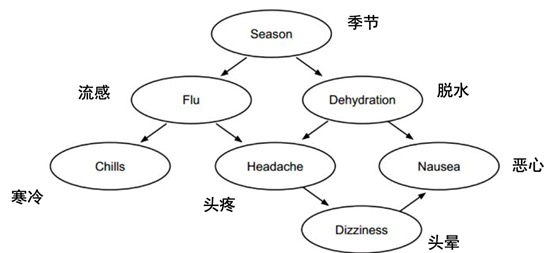
\includegraphics[width=0.5\textwidth]{images/title/贝叶斯网络.jpg}
		\caption{贝叶斯网络}
		\label{fig:贝叶斯网络}
	\end{figure}
	\vspace{-1cm}
	$$
	\left( \text{A} \right) .\,\, \textit{Season}\bot \textit{Chills}|\textit{Flu}\quad \left( \text{B} \right) .\,\, \textit{Season}\bot \textit{Chills}\quad \left( \text{C} \right) .\,\, \textit{Season}\bot \textit{Headache}|\textit{Flu}
	$$
	\solution 为了叙述方便, 我们不妨先对上述贝叶斯网络中的各节点进行拓扑排序, 具体如下图\ref{fig:简化后的贝叶斯网络}所示:
	\begin{figure}[H]  % 这里记得用[H]
		\centering
		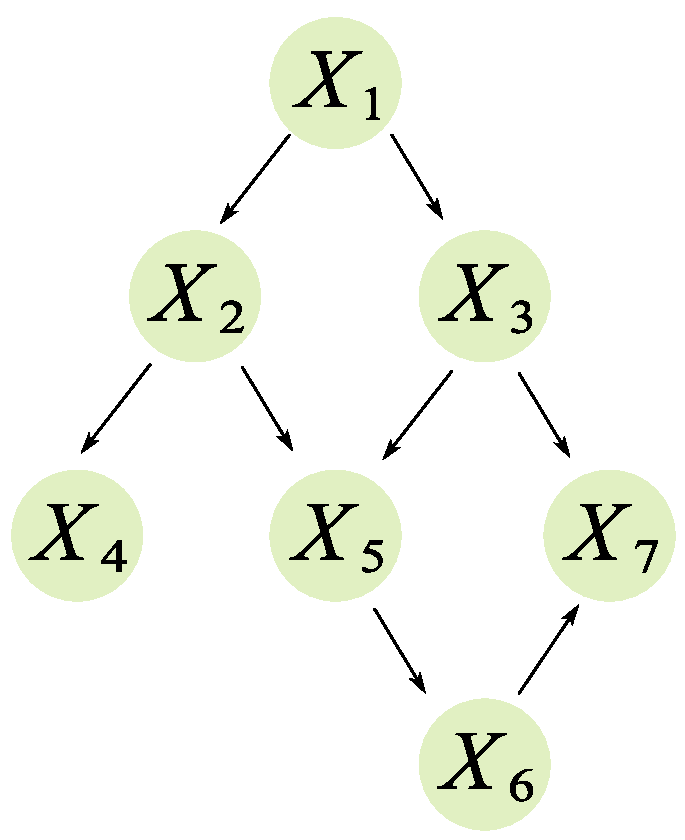
\includegraphics[width=0.2\textwidth]{images/title/简化后的贝叶斯网络.pdf}
		\caption{简化后的贝叶斯网络}
		\label{fig:简化后的贝叶斯网络}
	\end{figure}
	上述选项即变为
	$$
	\left( \text{A} \right) . X_1\bot X_4|X_2\quad \left( \text{B} \right) . X_1\bot X_4\quad \left( \text{C} \right) . X_1\bot X_5|X_2
	$$
	显然B选项错误, 先看C选项: 给定$X_2$时, 检查$X_1,X_5$的可达性. 利用快速检验准则: 从$X_1$出发, 通过$X_3$, 即可到达$X_5$, 因此C项错误. 再看A项, 利用准则可以看出, 从$X_1$出发, 要么在$X_1\to X_2\to X_4$这条路线上被反弹回$X_1$. 要么先经过$X_1\to X_3\to X_5$到达$X_5$, 但是球在路线$X_5\to X_2\to X_4$上被$X_2$截止了, 总之到达不了$X_4$; 从$X_4$出发, 类似的, 也是到达不了$X_1$. 因此, $X_1\bot X_4|X_2$(即A项正确).
\end{homeworkProblem}

\pagebreak

\begin{homeworkProblem}
	已知以下贝叶斯网络(如图\ref{fig:贝叶斯网络2}中所示), 包含4个二值变量, 则该网络一共有(\quad)个参数.

	\begin{figure}[H]  % 这里记得用[H]
		\centering
		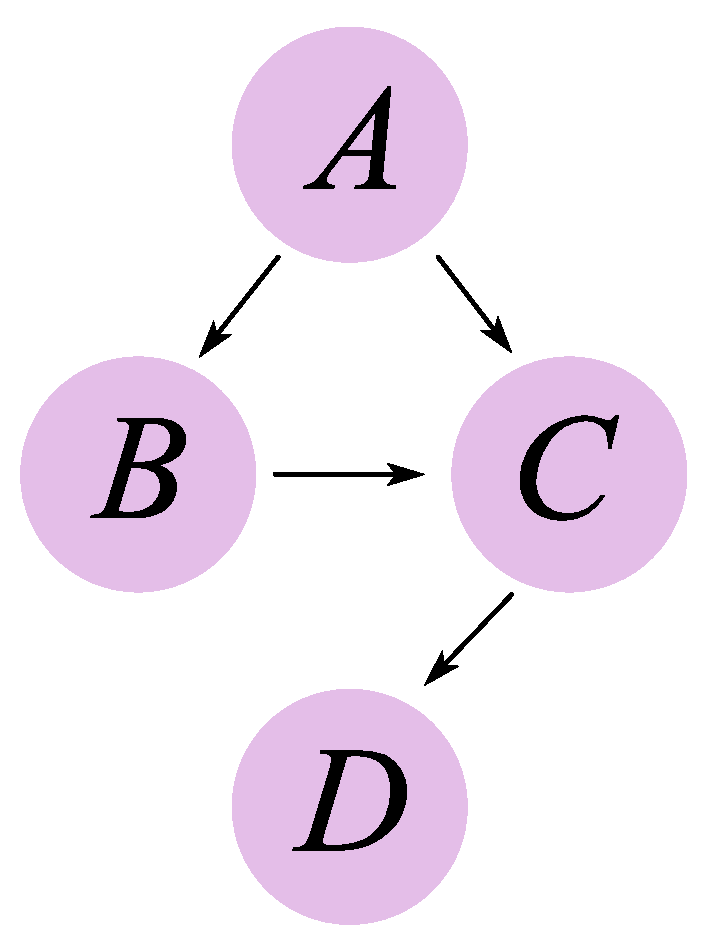
\includegraphics[width=0.2\textwidth]{images/title/贝叶斯网络2.pdf}
		\caption{贝叶斯网络}
		\label{fig:贝叶斯网络2}
	\end{figure}
	\solution 先写出联合概率分布$$p\left( A,B,C,D \right) =p\left( A \right) \cdot p\left( B|A \right) \cdot p\left( C|A,B \right) \cdot p\left( D|C \right) 
	$$
	因此网络参数共有$2^0+2^1+2^2+2^1=9$个, 于是选C项.
\end{homeworkProblem}



\begin{homeworkProblem}
	假设你有3个盒子, 每个盒子里都有一定数量的苹果和橘子. 每次随机选择一个盒子, 然后从盒子里选一个水果, 并记录你的发现($a$代表苹果, $o$代表橘子). 不幸的是, 你忘了写下你所选的盒子, 只是简单的记下了苹果和橘子. 假设每个盒子中水果数量如下:
	\begin{itemize}
		\item 盒子1: 2个苹果, 2个橘子;
		\item 盒子2: 3个苹果, 1个橘子;
		\item 盒子3: 1个苹果, 3个橘子;
	\end{itemize}
	
	(1). 请用HMM模型描述上述过程;

	(2). 请给出水果序列$\boldsymbol{x}=\left( a,a,o,o,o \right) $对应的最佳盒子序列.

	\solution \,\,(1).将盒子视作隐变量(即状态节点), 拿出来的水果视作观测变量(即输出节点). 因为每次都是随机选取的盒子, 因此初始状态的概率分布应为均匀分布, 即$\boldsymbol{\pi }=\left( \begin{matrix}
		1/3&		1/3&		1/3\\
	\end{matrix} \right) ^{\text{T}}$. 因为每次都是以均匀分布抽取盒子的且$a_{ij}=p\left( y_{t+1}=s_j|y_t=s_i \right) $, 因此盒子间的状态转移矩阵为$$\boldsymbol{A}=\left( a_{ij} \right) _{N\times N}=\left( \begin{matrix}
		1/3&		1/3&		1/3\\
		1/3&		1/3&		1/3\\
		1/3&		1/3&		1/3\\
	\end{matrix} \right)$$
	由于$b_{ij}=p\left( x_t=o_j|y_t=s_i \right)$, 因此发射概率矩阵(给定盒子时, 选择每种水果的概率)为$$\boldsymbol{B}=\left( b_{ij} \right) _{N\times M}=\left( \begin{matrix}
		1/2&		1/2\\
		3/4&		1/4\\
		1/4&		3/4\\
	\end{matrix} \right) $$

	(2). Viterbi解码算法如下:
	{\color{red}
	\begin{align}
		&\text{动态规划}: V_1\left( j \right) =\pi _jb_j\left( x_1 \right) ,\begin{cases}
			V_t\left( j \right) =b_j\left( x_t \right) \cdot \underset{1\le i\le N}{\text{max}}\left\{ a_{ij}V_{t-1}\left( i \right) \right\}\\
			\psi _t\left( j \right) =\text{arg} \underset{1\le i\le N}{\text{max}}\left\{ a_{ij}V_{t-1}\left( i \right) \right\}\\
		\end{cases},\text{其中}1\le j\le N \notag
		\\
		&\text{反向回溯}: P^{\ast}=\underset{1\le i\le N}{\text{max}}V_T\left( i \right) ,\begin{cases}
			i_{T}^{\ast}=\text{arg} \underset{1\le i\le N}{\text{max}}V_T\left( i \right)\\
			i_{t}^{\ast}=\psi _{t+1}\left( i_{t+1}^{\ast} \right)\\ 
		\end{cases} \notag
	\end{align}
	}
	\begin{itemize}
		\item 当$t=1$时, 已知$x_1=a$, 所以初始化如下:
		\begin{align}
			V_1\left( 1 \right) &=\pi _1b_1\left( a \right) =1/3\cdot 1/2=1/6 ,\psi_1(1)=0 \notag
			\\
			V_1\left( 2 \right) &=\pi _2b_2\left( a \right) =1/3\cdot 3/4=1/4 ,\psi_1(2)=0 \notag
			\\
			V_1\left( 3 \right) &=\pi _3b_3\left( a \right) =1/3\cdot 1/4=1/12 ,\psi_1(3)=0 \notag
		\end{align}
		\item 当$t=2$时, 已知$x_2=a$, 所以有:
		\begin{align}
			V_2\left( 1 \right) &=b_1\left( a \right) \cdot 1/3\cdot 1/4=1/24,\psi _2\left( 1 \right) =2 \notag
			\\
			V_2\left( 2 \right) &=b_2\left( a \right) \cdot 1/3\cdot 1/4=1/16,\psi _2\left( 2 \right) =2 \notag
			\\
			V_2\left( 3 \right) &=b_3\left( a \right) \cdot 1/3\cdot 1/4=1/48,\psi _2\left( 3 \right) =2 \notag
		\end{align}
		\item 当$t=3$时, 已知$x_3=o$, 所以有:
		\begin{align}
			V_3\left( 1 \right) &=b_1\left( o \right) \cdot 1/3\cdot 1/16=1/96,\psi _3\left( 1 \right) =2 \notag
			\\
			V_3\left( 2 \right) &=b_2\left( o \right) \cdot 1/3\cdot 1/16=1/192,\psi _3\left( 2 \right) =2 \notag
			\\
			V_3\left( 3 \right) &=b_3\left( o \right) \cdot 1/3\cdot 1/16=1/64,\psi _3\left( 3 \right) =2 \notag
		\end{align}
		\item 当$t=4$时, 已知$x_4=o$, 所以有:
		\begin{align}
			V_4\left( 1 \right) &=b_1\left( o \right) \cdot 1/3\cdot 1/64=1/384,\psi _4\left( 1 \right) =3 \notag
			\\
			V_4\left( 2 \right) &=b_2\left( o \right) \cdot 1/3\cdot 1/64=1/768,\psi _4\left( 2 \right) =3 \notag
			\\
			V_4\left( 3 \right) &=b_3\left( o \right) \cdot 1/3\cdot 1/64=1/256,\psi _4\left( 3 \right) =3 \notag
		\end{align}
		\item 当$t=5$时, 已知$x_5=o$, 所以有:
		\begin{align}
			V_5\left( 1 \right) &=b_1\left( o \right) \cdot 1/3\cdot 1/256=1/1536,\psi _5\left( 1 \right) =3 \notag
			\\
			V_5\left( 2 \right) &=b_2\left( o \right) \cdot 1/3\cdot 1/256=1/3072,\psi _5\left( 2 \right) =3 \notag
			\\
			V_5\left( 3 \right) &=b_3\left( o \right) \cdot 1/3\cdot 1/256=1/1024,\psi _5\left( 3 \right) =3 \notag
		\end{align}
	\end{itemize}
	迭代过程终止, 且$\displaystyle P^{\ast}=\underset{1\le i\le 3}{\text{max}}V_{T}(i)=V_{5}(3)=\frac{1}{1024}$. 回溯过程为:$$i_{5}^{\ast}=3,i_{4}^{\ast}=\psi _5\left( 3 \right) =3,i_{3}^{\ast}=\psi _4\left( 3 \right) =3,i_{2}^{\ast}=\psi _3\left( 3 \right) =2,i_{1}^{\ast}=\psi _2\left( 2 \right) =2
	$$
	因此回溯出最优路径为$\boldsymbol{y}=\left\{ 2,2,3,3,3 \right\}$.
\end{homeworkProblem}
\newpage

\begin{homeworkProblem}
	给定如图\ref{fig:HMM}所示的HMM
	\begin{figure}[H]  % 这里记得用[H]
		\centering
		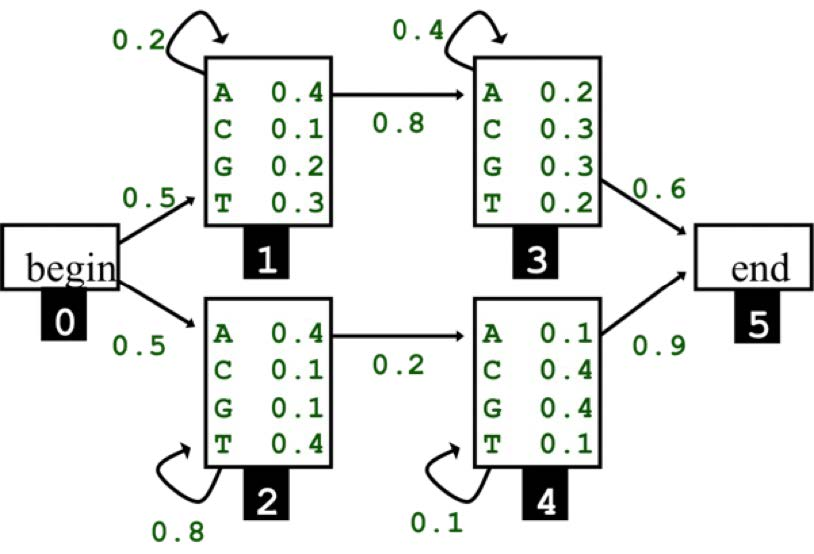
\includegraphics[width=0.5\textwidth]{images/title/HMM.jpg}
		\caption{HMM示意图}
		\label{fig:HMM}
	\end{figure}
	(1). 采用前向算法计算序列AGTT出现概率;

	(2). 计算观测TATA最可能的序列.

	\solution \,\,(1). 由于初始状态节点已经确定为“0”了, 所以初始状态的概率分布为$$\boldsymbol{\pi }=\left( 1,0,0,0,0,0 \right) ^{\text{T}}$$
	转移概率矩阵$\boldsymbol{A}$和发射概率矩阵$\boldsymbol{B}$(把begin和end也看做观测状态且放到$\boldsymbol{B}$的最后两列)分别为:
	$$
	\boldsymbol{A}=\left( \begin{matrix}
		0&		0.5&		0.5&		0&		0&		0\\
		0&		0.2&		0&		0.8&		0&		0\\
		0&		0&		0.8&		0&		0.2&		0\\
		0&		0&		0&		0.4&		0&		0.6\\
		0&		0&		0&		0&		0.1&		0.9\\
		0&		0&		0&		0&		0&		1\\
	\end{matrix} \right) ,\boldsymbol{B}=\left( \begin{matrix}
		0&		0&		0&		0&		1&		0\\
		0.4&		0.1&		0.2&		0.3&		0&		0\\
		0.4&		0.1&		0.1&		0.4&		0&		0\\
		0.2&		0.3&		0.3&		0.2&		0&		0\\
		0.1&		0.4&		0.4&		0.1&		0&		0\\
		0&		0&		0&		0&		0&		1\\
	\end{matrix} \right) 
	$$

	$\alpha$递归计算的前向算法为:
	$$
	{\color{red}
	\alpha _1\left( j \right) =\pi _jb_j\left( x_1 \right) ,\alpha _t\left( j \right) =b_j\left( x_t \right) \cdot \sum_{i=1}^N{a_{ij}\alpha _{t-1}\left( i \right)},\text{其中}1\le j\le N
	} 
	$$
	
	为叙述方便, 将状态“0,1,2,3,4,5”记作状态“1,2,3,4,5,6”. 此时观测序列为$\left\{ \text{begin},A,G,T,T,\text{end} \right\}$.
	
	因此初始化($t=1$时), 则有$x_1=\text{begin}$且:
	\begin{align}
		\alpha _1\left( 1 \right) =\pi _1b_1\left( x_1 \right) =1\cdot 1=1,\alpha _1\left( 2 \right) =\alpha _1\left( 3 \right) =\alpha _1\left( 4 \right) =\alpha _1\left( 5 \right) =\alpha _1\left( 6 \right) =0 \notag
	\end{align}

	当$t=2$时, 则有$\displaystyle x_2=A,\alpha _2\left( j \right) =b_j\left( A \right) \cdot \sum_{i=1}^6{a_{ij}\alpha _1\left( i \right)}	$且:
	$$
	\alpha _2\left( 1 \right) =0,\alpha _2\left( 2 \right) =0.2,\alpha _2\left( 3 \right) =0.2,\alpha _2\left( 4 \right) =0,\alpha _2\left( 5 \right) =0,\alpha _2\left( 6 \right) =0
	$$

	当$t=3$时, 则有$\displaystyle x_3=G,\alpha _3\left( j \right) =\left( \sum_{i=1}^6{\alpha _2\left( i \right) a_{ij}} \right) b_j\left( G \right)$且:
	$$
	\alpha _3\left( 1 \right) =0,\alpha _3\left( 2 \right) =0.008,\alpha _3\left( 3 \right) =0.016,\alpha _3\left( 4 \right) =0.048,\alpha _3\left( 5 \right) =0.016,\alpha _3\left( 6 \right) =0
	$$

	当$t=4$时, 则有$\displaystyle x_4=T,\alpha _4\left( j \right) =\left( \sum_{i=1}^6{\alpha _3\left( i \right) a_{ij}} \right) b_j\left( T \right)$且:
	$$
	\alpha _4\left( 1 \right) =0,\alpha _4\left( 2 \right) =0.00048,\alpha _4\left( 3 \right) =0.00512,\alpha _4\left( 4 \right) =0.00512,\alpha _4\left( 5 \right) =0.00048,\alpha _4\left( 6 \right) =0
	$$

	当$t=5$时, 则有$\displaystyle x_5=T,\alpha _5\left( j \right) =\left( \sum_{i=1}^6{\alpha _4\left( i \right) a_{ij}} \right) b_j\left( T \right)$且:
	$$
	\alpha _5\left( 1 \right) =0,\alpha _5\left( 2 \right) =0.0000288,\alpha _5\left( 3 \right) =0.00164,\alpha _5\left( 4 \right) =0.000486,\alpha _5\left( 5 \right) =0.000107,\alpha _5\left( 6 \right) =0
	$$

	当$t=6$时, 则有$\displaystyle x_6=\text{end},\alpha _6\left( j \right) =\left( \sum_{i=1}^6{\alpha _5\left( i \right) a_{ij}} \right) b_j\left( \text{end} \right)$且:
	$$
	\alpha _6\left( 1 \right) =\alpha _5\left( 2 \right) =\alpha _5\left( 3 \right) =\alpha _5\left( 4 \right) =\alpha _5\left( 5 \right) =0,\alpha _5\left( 6 \right) =0.000388
	$$

	因此序列$(x_1,x_2,x_3,x_4,x_5,x_6)=(\text{begin,A,G,T,T,end})$的出现概率为
	$$
	p\left( x_1,x_2,x_3,x_4,x_5,x_6|\boldsymbol{A},\boldsymbol{B},\boldsymbol{\pi } \right) =\sum_{j=1}^6{\alpha _6\left( j \right)}=0.000388
	$$

	(2). 注意到观测序列为$\left\{ \text{begin},T,A,T,A,\text{end} \right\}$, Viterbi解码算法如下:
	{\color{red}
	\begin{align}
		&\text{动态规划}: V_1\left( j \right) =\pi _jb_j\left( x_1 \right) ,\begin{cases}
			V_t\left( j \right) =b_j\left( x_t \right) \cdot \underset{1\le i\le N}{\text{max}}\left\{ a_{ij}V_{t-1}\left( i \right) \right\}\\
			\psi _t\left( j \right) =\text{arg} \underset{1\le i\le N}{\text{max}}\left\{ a_{ij}V_{t-1}\left( i \right) \right\}\\
		\end{cases},\text{其中}1\le j\le N \notag
		\\
		&\text{反向回溯}: P^{\ast}=\underset{1\le i\le N}{\text{max}}V_T\left( i \right) ,\begin{cases}
			i_{T}^{\ast}=\text{arg} \underset{1\le i\le N}{\text{max}}V_T\left( i \right)\\
			i_{t}^{\ast}=\psi _{t+1}\left( i_{t+1}^{\ast} \right)\\ 
		\end{cases} \notag
	\end{align}
	}
	\begin{itemize}
		\item 当$t=1$时, 已知$x_1=\text{begin}$, 所以初始化如下:
		\begin{align}
			V_1\left( 1 \right) &=1,V_1\left( 2 \right) =V_1\left( 3 \right) =V_1\left( 4 \right) =V_1\left( 5 \right) =V_1\left( 6 \right) =0 \notag
			\\
			\psi _1\left( 1 \right) &=\psi _1\left( 2 \right) =\psi _1\left( 3 \right) =\psi _1\left( 4 \right) =\psi _1\left( 5 \right) =\psi _1\left( 6 \right) =0 \notag
		\end{align}
		\item 当$t=2$时, 已知$x_2=T$, 所以有:
		\begin{align}
			V_2\left( 1 \right) &=0,V_2\left( 2 \right) =0.15,V_2\left( 3 \right) =0.2,V_2\left( 4 \right) =0,V_2\left( 5 \right) =0,V_2\left( 6 \right) =0 \notag
			\\
			\psi _2\left( 1 \right) &=1,\psi _2\left( 2 \right) =1,\psi _2\left( 3 \right) =1,\psi _2\left( 4 \right) =1,\psi _2\left( 5 \right) =1, \psi _2\left( 6 \right) =1 \notag
		\end{align}
		\item 当$t=3$时, 已知$x_3=A$, 所以有:
		\begin{align}
			&V_3\left( 1 \right) =0,V_3\left( 2 \right) =0.012,V_3\left( 3 \right) =0.064,V_3\left( 4 \right) =0.024,V_3\left( 5 \right) =0.004,V_3\left( 6 \right) =0 \notag
			\\
			&\psi _3\left( 1 \right) =1,\psi _3\left( 2 \right) =2,\psi _3\left( 3 \right) =3,\psi _3\left( 4 \right) =2,\psi _3\left( 5 \right) =3,\psi _3\left( 6 \right) =1 \notag
		\end{align}
		\item 当$t=4$时, 已知$x_4=T$, 所以有:
		\begin{align}
			&V_4\left( 1 \right) =0,V_4\left( 2 \right) =0.00072,V_4\left( 3 \right) =0.02048,V_4\left( 4 \right) =0.00192,V_4\left( 5 \right) =0.00128,V_4\left( 6 \right) =0 \notag
			\\
			&\psi _4\left( 1 \right) =1,\psi _4\left( 2 \right) =2,\psi _4\left( 3 \right) =3,\psi _4\left( 4 \right) =2,\psi _4\left( 5 \right) =3,\psi _4\left( 6 \right) =4 \notag
		\end{align}
		\item 当$t=5$时, 已知$x_5=T$, 所以有:
		\begin{align}
			&V_5\left( 1 \right) =0,V_5\left( 2 \right) =5.76\times 10^{-5},V_5\left( 3 \right) =0.0065536,V_5\left( 4 \right) =0.0001536,V_5\left( 5 \right) =0.0004096,V_5\left( 6 \right) =0 \notag
			\\
			&\psi _5\left( 1 \right) =1,\psi _5\left( 2 \right) =2,\psi _5\left( 3 \right) =3,\psi _5\left( 4 \right) =4,\psi _5\left( 5 \right) =3,\psi _5\left( 6 \right) =5 \notag
		\end{align}
		\item 当$t=6$时, 已知$x_6=\text{end}$, 所以有:
		\begin{align}
			&V_6\left( 1 \right) =0,V_6\left( 2 \right) =0,V_6\left( 3 \right) =0,V_6\left( 4 \right) =0,V_6\left( 5 \right) =0,V_6\left( 6 \right) =0.00036864 \notag
			\\
			&\psi _6\left( 1 \right) =1,\psi _6\left( 2 \right) =2,\psi _6\left( 3 \right) =3,\psi _6\left( 4 \right) =4,\psi _6\left( 5 \right) =3,\psi _6\left( 6 \right) =5 \notag
		\end{align}
	\end{itemize}
	迭代过程终止, 且$\displaystyle P^{\ast}=\underset{1\le i\le 4}{\text{max}}V_{T}^{i}=V_{6}(6)=0.00036864,i_{6}^{\ast}=6$, 于是回溯过程如下:
	\begin{align}
		&i_{6}^{\ast}=\text{arg} \underset{1\le i\le 6}{\text{max}}V_6\left( i \right) =6,i_{5}^{\ast}=\psi _6\left( i_{6}^{\ast} \right) =\psi _6\left( 6 \right) =5,i_{4}^{\ast}=\psi _5\left( i_{5}^{\ast} \right) =\psi _5\left( 5 \right) =3, \notag
		\\
		&i_{3}^{\ast}=\psi _4\left( i_{4}^{\ast} \right) =\psi _4\left( 3 \right) =3,i_{2}^{\ast}=\psi _3\left( i_{3}^{\ast} \right) =\psi _3\left( 3 \right) =3,i_{1}^{\ast}=\psi _2\left( i_{2}^{\ast} \right) =\psi _2\left( 3 \right) =1 \notag
	\end{align}
	因此回溯得到的最优序列为$1\to 3 \to 3 \to 3 \to 5 \to 6$, 将标号对应回去则\textbf{真正的最优序列}为$0\to 2 \to 2 \to 2 \to 4 \to 5$, 且对应的概率值为$0.00036864$.

	接下来我们需要通过实验代码来验证上述计算的正确性, 因此我们需要先给出其伪代码:
	\begin{algorithm}[H]
		\begin{algorithmic}[1]
		\Require{转移概率矩阵$\boldsymbol{A}$, 发射概率矩阵$B$, 初始概率分布$\boldsymbol{\pi}$}
		\Ensure{HMM的最优路径}
		\State $\textbf{Viterbi}(\boldsymbol{A},\boldsymbol{B},\boldsymbol{\pi})$\textbf{:}
			\For{$j\gets 1$; $j \leq N$; $j\gets j+1$}
				\State $\psi _1\left( j \right) \gets 0$;
				\State $V_1\left( j \right) \gets \pi _jb_j\left( x_1 \right) $; \Comment{$t=1$时的初始化, 其中$b_j\left( x_t \right)$为状态节点$j$输出$x_t$的概率}
			\EndFor
			\For{$t\gets 2$; $t\leq T$; $t\gets t+1$} \Comment{前向动态规划}
				\For{$j\gets 1$; $j \leq N$; $j\gets j+1$}
					\State $\displaystyle V_t\left( j \right) =b_j\left( x_t \right) \cdot \underset{1\le i\le N}{\text{max}}\left\{ a_{ij}V_{t-1}\left( i \right) \right\}$;
					\State $\displaystyle \psi _t\left( j \right) =\text{arg} \underset{1\le i\le N}{\text{max}}\left\{ a_{ij}V_{t-1}\left( i \right) \right\}$;
				\EndFor
			\EndFor
			\State $\displaystyle P^{\ast}\gets \underset{1\le i\le N}{\text{max}}V_T\left( i \right) ,i_{T}^{\ast}\gets \text{arg} \underset{1\le i\le N}{\text{max}}V_T\left( i \right)$; \Comment{初始化反向回溯}
			\For{$t\gets T -1$; $t\geq 1$; $t\gets t- 1$}
				\State $i_{t}^{\ast}=\psi _{t+1}\left( i_{t+1}^{\ast} \right)$; \Comment{反向状态回溯}
			\EndFor
			\State \Return 最优路径$\left\{ i_{1}^{\ast},i_{2}^{\ast},\cdots ,i_{T}^{\ast} \right\} $;
			\State \textbf{end \{Viterbi\}}
		\end{algorithmic}
		\caption{HMM状态序列解码的Viterbi算法}
		\label{alg:AdaBoost}
	\end{algorithm}
	现在分析一下算法的时间复杂度\footnote{伪码的8,9,12行需要一次for循环(循环变量为$i$)来求出最大值和所在索引, 需要消耗$O(N)$的时间.}, $T(N,T)=O(N)+O(T\cdot N\cdot N)+O(N)=O(T\cdot N^2)$, 显然是多项式时间内可计算的. 有了上述伪码, 则可以写出本题的C++代码(如后页所示):
	\newpage

\begin{tcblisting}{listing engine=minted,boxrule=0.1mm,
colback=blue!5!white,colframe=blue!75!black,
listing only,left=5mm,enhanced,sharp corners=all,
overlay={\begin{tcbclipinterior}\fill[red!20!blue!20!white] (frame.south west)
rectangle ([xshift=5mm]frame.north west);\end{tcbclipinterior}},
minted language=c++,
minted style=tango,
minted options={fontsize=\small,breaklines,autogobble,linenos,numbersep=3mm}}
#include <bits/stdc++.h>
using namespace std;

int Idx(string x) {
    int res;
    if (x == "A") res = 0;
    else if (x == "C") res = 1;
    else if (x == "G") res = 2;
    else if (x == "T") res = 3;
    else if (x == "begin") res = 4;
    else if (x == "end") res = 5;
    return res;
}

vector<int> Viterbi( //Viterbi动态规划解码算法
    vector<string> &X, vector<double> &pi,
    vector<vector<double>> &A, vector<vector<double>> &B
) {
    int T = X.size(), N = A.size(), M = B[0].size();
    vector<vector<double>> V(T, vector<double>(N, 0));
    vector<vector<int>> psi(T, vector<int>(N, 0));
    for(int j = 0; j < N; j++) {
        V[0][j] = pi[j] * B[j][Idx(X[0])];
        psi[0][j] = 0;
    }
    for(int t = 1; t < T; t++) {
        for(int j = 0; j < N; j++) {
            double temp = A[0][j] * V[t - 1][0];
            int idx = 0;
            for(int i = 1; i < N; i++) {
                if(A[i][j] * V[t - 1][i] > temp) {
                    temp = A[i][j] * V[t - 1][i];
                    idx = i;
                }
            }
            V[t][j] = B[j][Idx(X[t])] * temp;
            psi[t][j] = idx;
        }
    }
    double P = V[T - 1][0];
    vector<int> path(T);
    for(int i = 1; i < N; i++) {
        if(V[T - 1][i] > P) {
            P = V[T - 1][i];
            path[T - 1] = i;
        }
    }
    for(int t = T - 2; t >= 0; t--) {
        path[t] = psi[t + 1][path[t + 1]];
    }
    return path;
}
\end{tcblisting}
主函数编码如下:
\begin{tcblisting}{listing engine=minted,boxrule=0.1mm,
colback=blue!5!white,colframe=blue!75!black,
listing only,left=5mm,enhanced,sharp corners=all,
overlay={\begin{tcbclipinterior}\fill[red!20!blue!20!white] (frame.south west)
rectangle ([xshift=5mm]frame.north west);\end{tcbclipinterior}},
minted language=c++,
minted style=tango,
minted options={fontsize=\small,breaklines,autogobble,linenos,numbersep=3mm}}
int main() {
    vector<string> X = {"begin", "T", "A", "T", "A", "end"};
    vector<double> pi = {1, 0, 0, 0, 0, 0};
    vector<vector<double>> A = {
        {0, 0.5, 0.5, 0, 0, 0},
        {0, 0.2, 0, 0.8, 0, 0},
        {0, 0, 0.8, 0, 0.2, 0},
        {0, 0, 0, 0.4, 0, 0.6},
        {0, 0, 0, 0, 0.1, 0.9},
        {0, 0, 0, 0, 0, 1}
    };
    vector<vector<double>> B = {
        {0, 0, 0, 0, 1, 0},
        {0.4, 0.1, 0.2, 0.3, 0, 0},
        {0.4, 0.1, 0.1, 0.4, 0, 0},
        {0.2, 0.3, 0.3, 0.2, 0, 0},
        {0.1, 0.4, 0.4, 0.1, 0, 0},
        {0, 0, 0, 0, 0, 1}
    };
    vector<int> path = Viterbi(X, pi, A, B);
    cout << "最优路径为: " << endl;
    for(int i = 0; i < path.size(); i++) {
        cout << path[i] << " ";
    }
}
\end{tcblisting}
相应的输出为:
\begin{tcblisting}{listing engine=minted,boxrule=0.1mm,
colback=blue!5!white,colframe=blue!75!black,
listing only,left=5mm,enhanced,sharp corners=all,
overlay={\begin{tcbclipinterior}\fill[red!20!blue!20!white] (frame.south west)
rectangle ([xshift=5mm]frame.north west);\end{tcbclipinterior}},
minted language=c++,
minted style=tango,
minted options={fontsize=\small,breaklines,autogobble,linenos,numbersep=3mm}}
开始运行...
最优路径为: 0 2 2 2 4 5 
运行结束
\end{tcblisting}
显然这与我们的手动计算结果是相同的, 证明了我们算法实现的正确性和手算的正确性.

并且我们可以利用python中的hmmlearn库来进行编码并输出最优序列, 具体代码如后页所示:
\begin{tcblisting}{listing engine=minted,boxrule=0.1mm,
colback=blue!5!white,colframe=blue!75!black,
listing only,left=5mm,enhanced,sharp corners=all,
overlay={\begin{tcbclipinterior}\fill[red!20!blue!20!white] (frame.south west)
rectangle ([xshift=5mm]frame.north west);\end{tcbclipinterior}},
minted language=python,
minted style=tango,
minted options={fontsize=\small,breaklines,autogobble,linenos,numbersep=3mm}}
# pip3 install hmmlearn
import numpy as np
from hmmlearn import hmm

states = ["0", "1", "2", "3", "4", "5"]
n_states = len(states)

observations = ["A", "C", "G", "T", "begin", "end"]
n_observations = len(observations)

start_probability = np.array([1, 0, 0, 0, 0, 0])

transition_probability = np.array([
    [0, 0.5, 0.5, 0, 0, 0],
    [0, 0.2, 0, 0.8, 0, 0],
    [0, 0, 0.8, 0, 0.2, 0],
    [0, 0, 0, 0.4, 0, 0.6],
    [0, 0, 0, 0, 0.1, 0.9],
    [0, 0, 0, 0, 0, 1]
])

emission_probability = np.array([
    [0, 0, 0, 0, 1, 0],
    [0.4, 0.1, 0.2, 0.3, 0, 0],
    [0.4, 0.1, 0.1, 0.4, 0, 0],
    [0.2, 0.3, 0.3, 0.2, 0, 0],
    [0.1, 0.4, 0.4, 0.1, 0, 0],
    [0, 0, 0, 0, 0, 1]
])

model = hmm.CategoricalHMM(n_components=n_states)
model.startprob_=start_probability
model.transmat_=transition_probability
model.emissionprob_=emission_probability

seen = np.array([[4, 3, 0, 3, 0, 5]]).T
logprob, box = model.decode(seen, algorithm="viterbi")
print("观测序列为:", ", ".join(map(lambda x: observations[x[0]], seen)))
print("最优路径为:", ", ".join(map(lambda x: states[x], box)))
\end{tcblisting}
上述代码的运行结果为:
\begin{tcblisting}{listing engine=minted,boxrule=0.1mm,
colback=blue!5!white,colframe=blue!75!black,
listing only,left=5mm,enhanced,sharp corners=all,
overlay={\begin{tcbclipinterior}\fill[red!20!blue!20!white] (frame.south west)
rectangle ([xshift=5mm]frame.north west);\end{tcbclipinterior}},
minted language=python,
minted style=tango,
minted options={fontsize=\small,breaklines,autogobble,linenos,numbersep=3mm}}
观测序列为: begin, T, A, T, A, end
最优路径为: 0, 2, 2, 2, 4, 5
\end{tcblisting}
由此可见, 自行编写的算法跟hmmlearn算法库的运行结果是一致的.
\end{homeworkProblem}

\pagebreak

\begin{homeworkProblem}
	请编写\textbf{Problem 4}中的C++程序和Python程序, 并展示运行结果.

	\solution \,\,C++代码如下所示:

\begin{tcblisting}{listing engine=minted,boxrule=0.1mm,
colback=blue!5!white,colframe=blue!75!black,
listing only,left=5mm,enhanced,sharp corners=all,
overlay={\begin{tcbclipinterior}\fill[red!20!blue!20!white] (frame.south west)
rectangle ([xshift=5mm]frame.north west);\end{tcbclipinterior}},
minted language=c++,
minted style=tango,
minted options={fontsize=\small,breaklines,autogobble,linenos,numbersep=3mm}}
#include <bits/stdc++.h>
using namespace std;

int Idx(string x) {
    int res;
    if (x == "Apple") res = 0;
    else if (x == "Orange") res = 1;
    return res;
}

vector<int> Viterbi( //Viterbi动态规划解码算法
    vector<string> &X, vector<double> &pi,
    vector<vector<double>> &A, vector<vector<double>> &B
) {
    int T = X.size(), N = A.size(), M = B[0].size();
    vector<vector<double>> V(T, vector<double>(N, 0));
    vector<vector<int>> psi(T, vector<int>(N, 0));
    for(int j = 0; j < N; j++) {
        V[0][j] = pi[j] * B[j][Idx(X[0])];
        psi[0][j] = 0;
    }
    for(int t = 1; t < T; t++) {
        for(int j = 0; j < N; j++) {
            double temp = A[0][j] * V[t - 1][0];
            int idx = 0;
            for(int i = 1; i < N; i++) {
                if(A[i][j] * V[t - 1][i] > temp) {
                    temp = A[i][j] * V[t - 1][i];
                    idx = i;
                }
            }
            V[t][j] = B[j][Idx(X[t])] * temp;
            psi[t][j] = idx;
        }
    }
    double P = V[T - 1][0];
    vector<int> path(T);
    for(int i = 1; i < N; i++) {
        if(V[T - 1][i] > P) {
            P = V[T - 1][i];
            path[T - 1] = i;
        }
    }
    for(int t = T - 2; t >= 0; t--) {
        path[t] = psi[t + 1][path[t + 1]];
    }
    return path;
}
\end{tcblisting}
主函数编码如下:
\begin{tcblisting}{listing engine=minted,boxrule=0.1mm,
colback=blue!5!white,colframe=blue!75!black,
listing only,left=5mm,enhanced,sharp corners=all,
overlay={\begin{tcbclipinterior}\fill[red!20!blue!20!white] (frame.south west)
rectangle ([xshift=5mm]frame.north west);\end{tcbclipinterior}},
minted language=c++,
minted style=tango,
minted options={fontsize=\small,breaklines,autogobble,linenos,numbersep=3mm}}
int main() {
    vector<string> X = {"Apple", "Apple", "Orange", "Orange", "Orange"};
    vector<double> pi = {1.0 / 3, 1.0 / 3, 1.0 / 3};
    vector<vector<double>> A = {
        {1.0 / 3, 1.0 / 3, 1.0 / 3},
        {1.0 / 3, 1.0 / 3, 1.0 / 3},
        {1.0 / 3, 1.0 / 3, 1.0 / 3}
    };
    vector<vector<double>> B = {
        {1.0 / 2, 1.0 / 2},
        {3.0 / 4, 1.0 / 4},
        {1.0 / 4, 3.0 / 4}
    };
    vector<int> path = Viterbi(X, pi, A, B);
    cout << "最优路径为: " ;
    for(int i = 0; i < path.size(); i++) {
        cout << path[i] + 1 << " ";
    }
}
\end{tcblisting}
代码输出结果为(即最优序列为盒子2$\to$盒子2$\to$盒子3$\to$盒子3$\to$盒子3):
\begin{tcblisting}{listing engine=minted,boxrule=0.1mm,
colback=blue!5!white,colframe=blue!75!black,
listing only,left=5mm,enhanced,sharp corners=all,
overlay={\begin{tcbclipinterior}\fill[red!20!blue!20!white] (frame.south west)
rectangle ([xshift=5mm]frame.north west);\end{tcbclipinterior}},
minted language=c++,
minted style=tango,
minted options={fontsize=\small,breaklines,autogobble,linenos,numbersep=3mm}}
开始运行...
最优路径为: 2 2 3 3 3 
运行结束
\end{tcblisting}
\textbf{Problem 4}和\textbf{Problem 5}的$\alpha$前向递归算法的C++代码如下所示:
\begin{tcblisting}{listing engine=minted,boxrule=0.1mm,
colback=blue!5!white,colframe=blue!75!black,
listing only,left=5mm,enhanced,sharp corners=all,
overlay={\begin{tcbclipinterior}\fill[red!20!blue!20!white] (frame.south west)
rectangle ([xshift=5mm]frame.north west);\end{tcbclipinterior}},
minted language=c++,
minted style=tango,
minted options={fontsize=\small,breaklines,autogobble,linenos,numbersep=3mm}}
double Forward_Alg( //alpha前向递归算法
    vector<string> &X, vector<double> &pi,
    vector<vector<double>> &A, vector<vector<double>> &B
) {
    int T = X.size(), N = A.size(), M = B[0].size();
    vector<vector<double>> alpha(T, vector<double>(N, 0));
    for(int j = 0; j < N; j++) {
        alpha[0][j] = pi[j] * B[j][Idx(X[0])];
    }
    for(int t = 1; t < T; t++) {
        for(int j = 0; j < N; j++) {
            double temp = 0;
            for(int i = 0; i < N; i++) {
               temp += A[i][j] * alpha[t - 1][i];
            }
            alpha[t][j] = B[j][Idx(X[t])] * temp;
        }
    }
    return accumulate(alpha[T - 1].begin(), alpha[T - 1].end(), 0.0);
}
\end{tcblisting}
主函数中添加如下代码并获得输出(显然跟手算结果是一样的, 因此代码正确):
\begin{tcblisting}{listing engine=minted,boxrule=0.1mm,
colback=blue!5!white,colframe=blue!75!black,
listing only,left=5mm,enhanced,sharp corners=all,
overlay={\begin{tcbclipinterior}\fill[red!20!blue!20!white] (frame.south west)
rectangle ([xshift=5mm]frame.north west);\end{tcbclipinterior}},
minted language=c++,
minted style=tango,
minted options={fontsize=\small,breaklines,autogobble,linenos,numbersep=3mm}}
vector<string> S = {"begin", "A", "G", "T", "T", "end"};
double prob = Forward_Alg(S, pi, A, B);
cout << "序列S的出现概率为" << prob << endl;
开始运行...
序列S的出现概率为0.00038832
运行结束
\end{tcblisting}
同时, Viterbi解码算法的Python代码如下:
\begin{tcblisting}{listing engine=minted,boxrule=0.1mm,
colback=blue!5!white,colframe=blue!75!black,
listing only,left=5mm,enhanced,sharp corners=all,
overlay={\begin{tcbclipinterior}\fill[red!20!blue!20!white] (frame.south west)
rectangle ([xshift=5mm]frame.north west);\end{tcbclipinterior}},
minted language=python,
minted style=tango,
minted options={fontsize=\small,breaklines,autogobble,linenos,numbersep=3mm}}
import numpy as np
from hmmlearn import hmm

states = ["盒子1", "盒子2", "盒子3"]
n_states = len(states)

observations = ["Apple", "Orange"]
n_observations = len(observations)

start_probability = np.array([1.0/3, 1.0/3, 1.0/3])

transition_probability = np.array([
    [1.0/3, 1.0/3, 1.0/3],
    [1.0/3, 1.0/3, 1.0/3],
    [1.0/3, 1.0/3, 1.0/3]
])

emission_probability = np.array([
    [1.0/2, 1.0/2],
    [3.0/4, 1.0/4],
    [1.0/4, 3.0/4]
])

model = hmm.CategoricalHMM(n_components=n_states)
model.startprob_=start_probability
model.transmat_=transition_probability
model.emissionprob_=emission_probability

seen = np.array([[0, 0, 1, 1, 1]]).T
logprob, box = model.decode(seen, algorithm="viterbi")
print("观测序列为:", ", ".join(map(lambda x: observations[x[0]], seen)))
print("最优路径为:", ", ".join(map(lambda x: states[x], box)))
\end{tcblisting}
代码输出为:
\begin{tcblisting}{listing engine=minted,boxrule=0.1mm,
colback=blue!5!white,colframe=blue!75!black,
listing only,left=5mm,enhanced,sharp corners=all,
overlay={\begin{tcbclipinterior}\fill[red!20!blue!20!white] (frame.south west)
rectangle ([xshift=5mm]frame.north west);\end{tcbclipinterior}},
minted language=python,
minted style=tango,
minted options={fontsize=\small,breaklines,autogobble,linenos,numbersep=3mm}}
观测序列为: Apple, Apple, Orange, Orange, Orange
最优路径为: 盒子2, 盒子2, 盒子3, 盒子3, 盒子3
\end{tcblisting}
\end{homeworkProblem}


% 引用文献
%\bibliographystyle{unsrt}  % unsrt:根据引用顺序编号
%\bibliography{refs}


\end{document}
